\chapter{Digital-Analog Wandler / Analog-Digital Wandler}
\textbf{Beispiel Musikspeicherung} \\
Schwallwellen $\rightarrow$ Mikrophon (Spannung - analoges Signal) $\rightarrow$ MP3-Datei (Bit 0/1 - digitales Signal) $\rightarrow$ DA-Wandler $\rightarrow$ Lautsprecher (analoges Signal)

\begin{figure}[H]
	\centering
	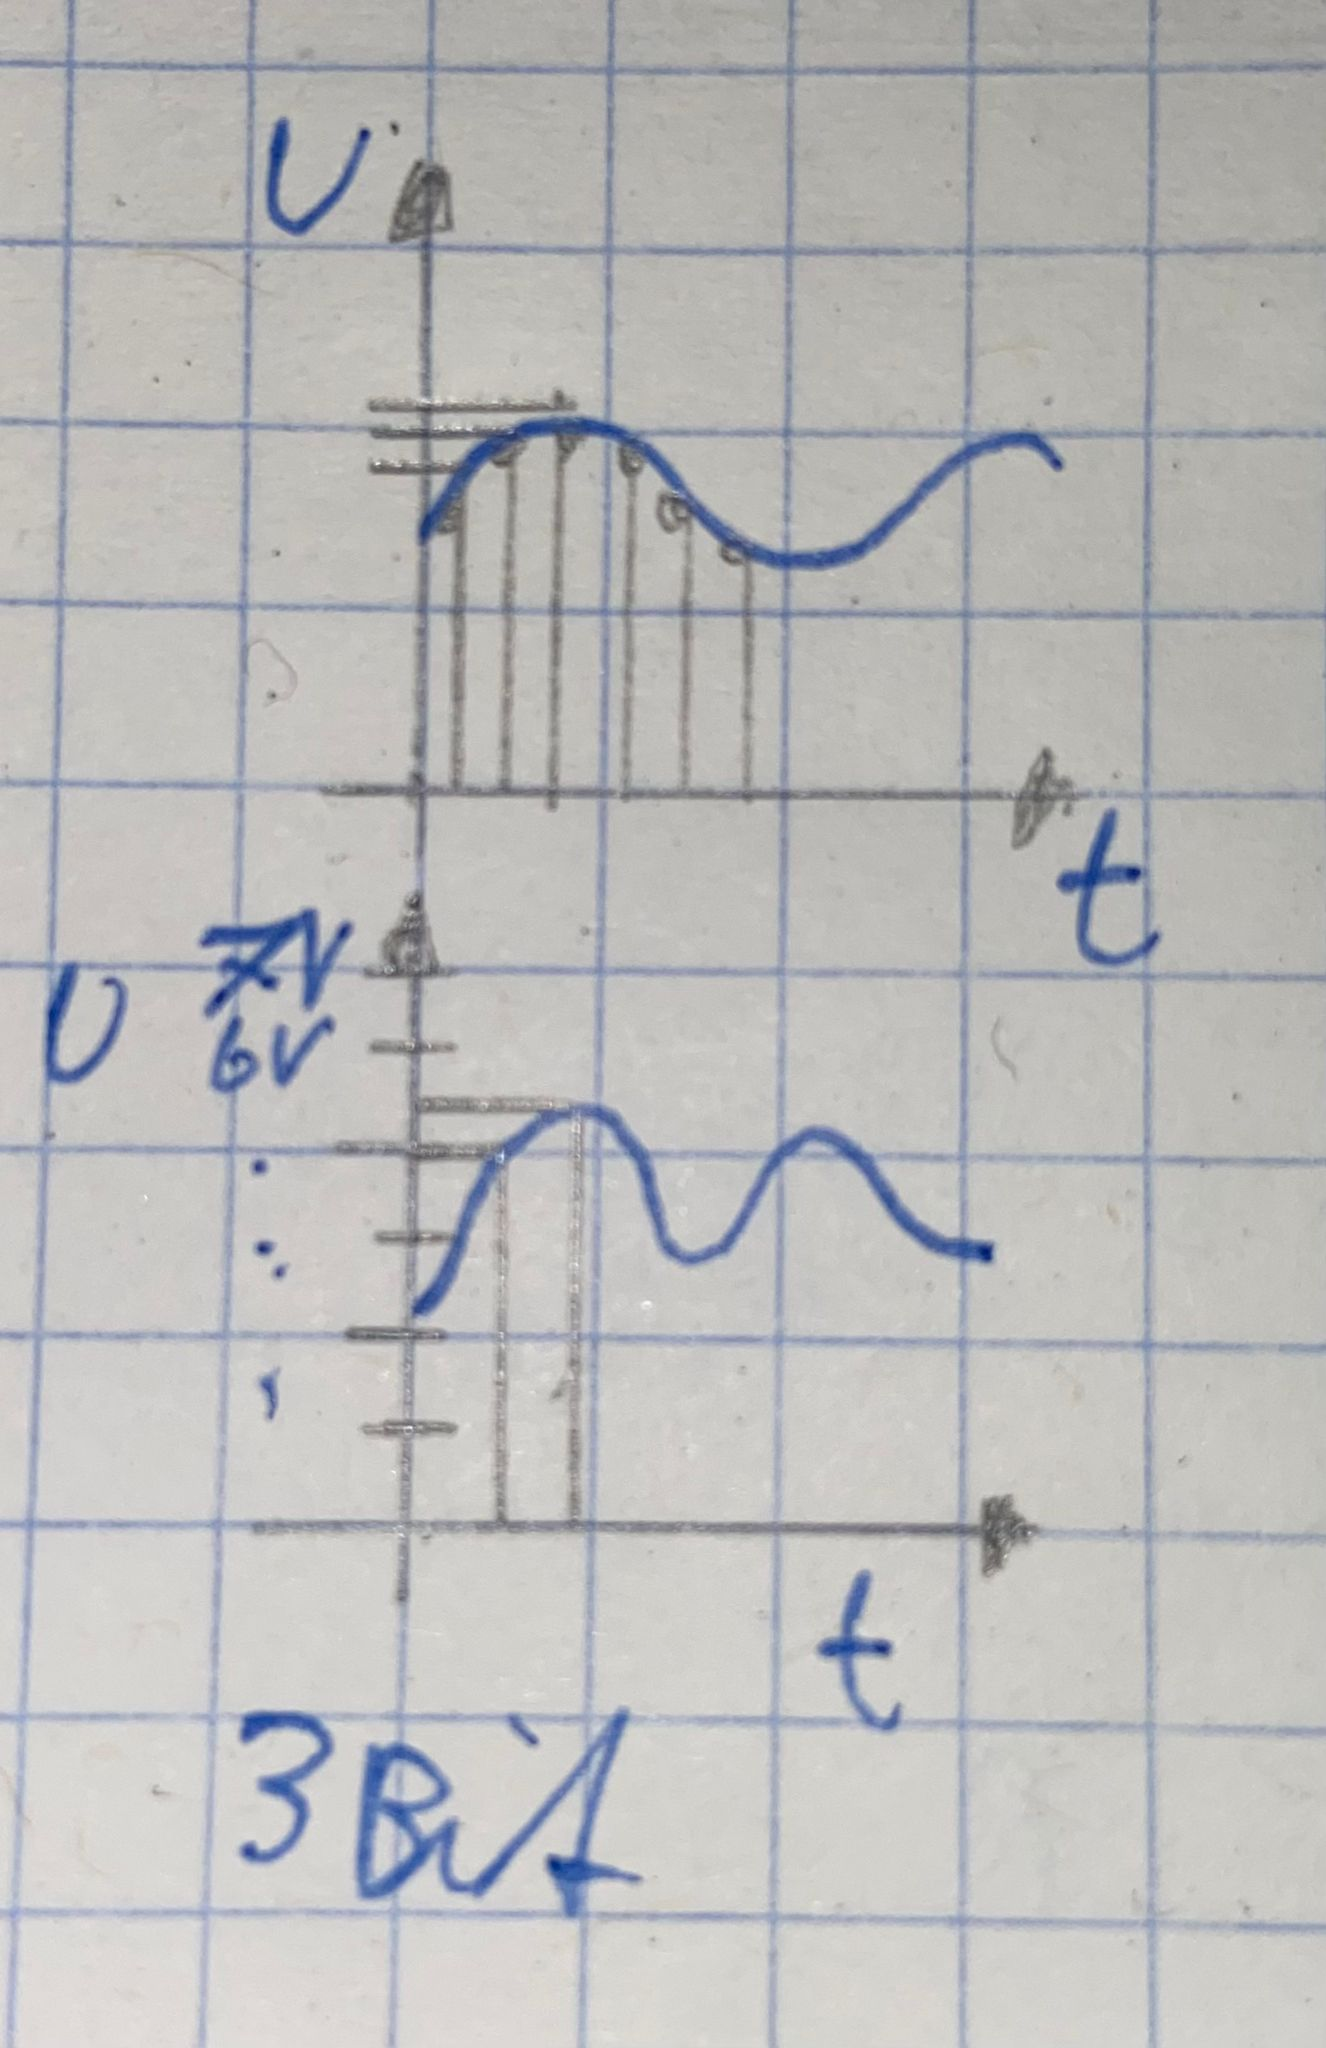
\includegraphics[width=0.2\linewidth]{figures/daad1.jpeg}
	\caption{DA/AD-Wandler}
\end{figure}

\begin{itemize}
	\item Pegel messen
	\item Binärzahl speichern
	\item je höher die Abtastrate (Samplerate) desto besser
	\item je mehr Bits zum Speichern verwendet werden, desto genauer
\end{itemize}
Typische Abtastrate: ca. 44 kHz

\section{Digital-Analog Wandler}
Aufgabe: muss aus einer Binärzahl eine Spannung erzeugen

Bsp: 2 Bit Spannung 0-5 Volt \\
00 $\rightarrow$ 0V \\
01 \\
10 \\
11 $\rightarrow$ 5V \\ \\
$\Rightarrow$ $\dfrac{5}{3}$ = $\Delta$U ... Schrittgröße
\begin{center}
	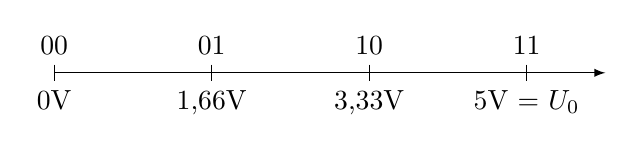
\begin{tikzpicture}
		\draw[-latex] (0,0) -- (7,0); %edit here for the axis
		\foreach \x in  {0,2,4,6} % edit here for the vertical lines
		\draw[shift={(\x,0)},color=black] (0pt,3pt) -- (0pt,-3pt);
		
		\draw (0,0) node[above=3pt]{00};
		\draw (2,0) node[above=3pt]{01};
		\draw (4,0) node[above=3pt]{10};
		\draw (6,0) node[above=3pt]{11};
		
		\draw (0,0) node[below=3pt]{0V};
		\draw (2,0) node[below=3pt]{1,66V};
		\draw (4,0) node[below=3pt]{3,33V};
		\draw (6,0) node[below=3pt]{5V = $\text{U}_0$};
	\end{tikzpicture}
\end{center}

Je mehr Bit, desto besser kann man den Spannungsbereich abdecken \\

\textbf{Allgemein:} Schrittgröße: $\Delta$U = $\dfrac{\text{U}_0}{2^{\text{n}}-1}$ \\
\textbf{maximaler Fehler:} $\text{F}_{\text{max}}$ = $\dfrac{\Delta \text{U}}{2}$

\textbf{Aufbau eines DA-Wandlers} \\
z.B. 3 Bit, $\text{U}_0$ = 5 Volt \\
zur Vereinfachung: $\Delta$U = $\dfrac{\text{U}_0}{2^{\text{n}}}$ statt $\Delta$U = $\dfrac{\text{U}_0}{2^{\text{n}}-1}$ \\

$\Delta$U = $\dfrac{5}{2^{3}}$ = $\dfrac{5}{8}$V = 0,625V

\begin{tabular}{|c|c|r|}
	\hline
	\textbf{Deziaml} & \textbf{Eingang} & \textbf{Ausgang} \\
	\hline
	0 & 000 & 0V \\ 
	\hline
	1 & 001 & 0,625V \\ 
	\hline
	2 & 010 & 1,25V \\ 
	\hline
	3 & 011 & 1,875V \\ 
	\hline
	4 & 100 & 2,5V \\ 
	\hline
	5 & 101 & 3,125V \\
	\hline
	6 & 110 & 3,75V \\
	\hline
	7 & 111 & 4,375V \\
	\hline
\end{tabular}

110 = 2,5 + 1,25 = 3,75V \\

\textbf{Schaltung eines DA-Wandlers} \\
\begin{figure}[H]
	\centering
	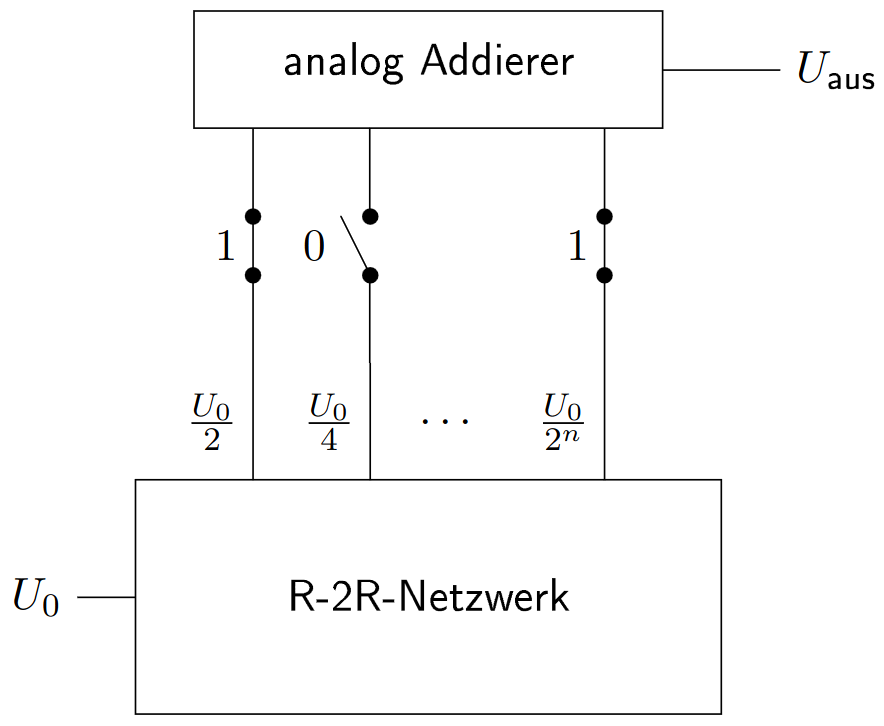
\includegraphics[width=0.8\linewidth]{figures/da_wandler.png}
	\caption{DA-Wandler}
\end{figure}

Schaltung wo die Spannung immer halbiert wird. \\
Idee: gleich große Widerstände in einer Reihenschaltung

\begin{figure}[H]
	\centering
	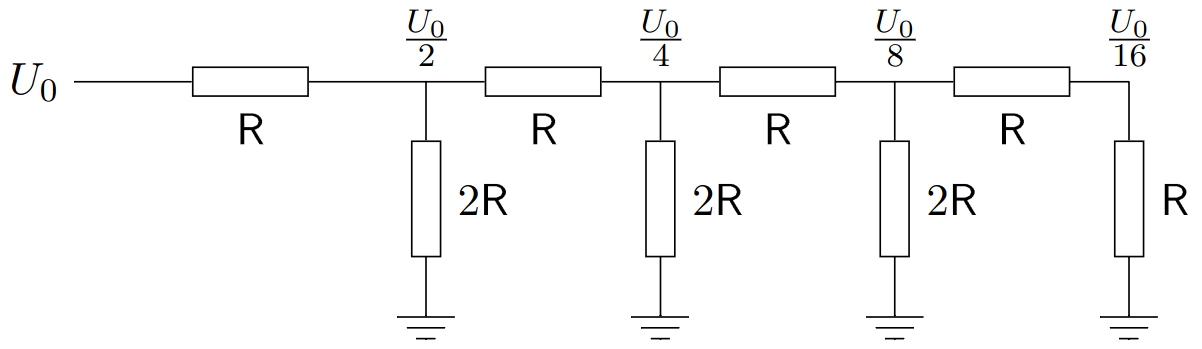
\includegraphics[width=0.8\linewidth]{figures/r2r.png}
	\caption{R-2R-Netzwerk}
\end{figure}

Beispiel: DA-Wandler 8 Bit, $\text{U}_0$ = 10V \\
\begin{enumerate}
	\item Wie groß ist eine Schrittgröße? ($\Delta$U) \\
	$\Delta$U = $\dfrac{10}{2^{8}}$ = 0,039625V
	\item Wie groß ist der maximale Fehler? \\
	$\text{F}_{\text{max}}$ = $\dfrac{0,039625}{2}$ = 0,01953125V (außer ganz oben bei 10V, $\Delta$U)
	\item Welche Spannung erzeugt die Eingabe von 10011101? \\
	$(\text{10011101})_2$ = $(\text{157})_{10}$ \\
	$\text{U}_{\text{aus}}$ = 157$\cdot$$\Delta$U = 6,221125V
	\item Welche Binärzahl wird für 8V verwendet und wie groß ist der Fehler? \\
	$\dfrac{8}{\Delta\text{U}}$ = $(\text{204,8})_{10}$ $\approx$ $(\text{205})_{10}$ = $(\text{11001101})_2$ \\ \\
	8V = x$\cdot$$\Delta$U $\Rightarrow$ 205$\cdot$$\Delta$U = 8,123125 \\
	Fehler = 8,123125 - 8 = 0,123125V
	\item Wei viele Bits benötigt man damit der Fehler kleiner als 2mVist? Wie groß ist der Fehler? \\
	n = ?, $\text{U}_0$ = 10V, $\text{F}_{\text{max}}$ $\le$ 2mV \\
	$\text{F}_{\text{max}}$ $\le$ 2mV \\
	$\dfrac{\Delta\text{U}}{2}$ = $\dfrac{\text{U}_0}{\dfrac{2^\text{n}}{2}}$ $\le$ 2mV \quad$\vert$ $\cdot$2 \\
	$\dfrac{\text{U}_0}{2^\text{n}}$ $\le$ 0,004 V \quad$\vert$ $\cdot$$2^\text{n}$ \quad$\vert$/0,004 \\
	$\dfrac{10}{0,004}$ = $2^\text{n}$ \quad ln \\
	ln(2500) = n$\cdot$ln(2) \quad$\vert$/ln(2) \\
	$\dfrac{ln(2500)}{ln(2)}$ = n \\
	11,2577 = n \\
	n $\approx$ 12 \\
	
	$\Delta$U = $\dfrac{\text{U}_0}{2^\text{n}}$ = $\dfrac{10}{2^{12}}$ = 2,44 mV \\
	
	$\text{F}_{\text{max}}$ = $\dfrac{ \dfrac{10}{2^{12}} }{2}$ = 1,22 mV

\end{enumerate}

\section{Analog-Digital Wandler}
Der Analog-Digital Wandler muss beliebige Werte (analoges Signal) in eine Binärzahl übersetzen.
